%%GNUPLOT: LaTeX picture with Postscript
%\begin{picture}(0,0)%
%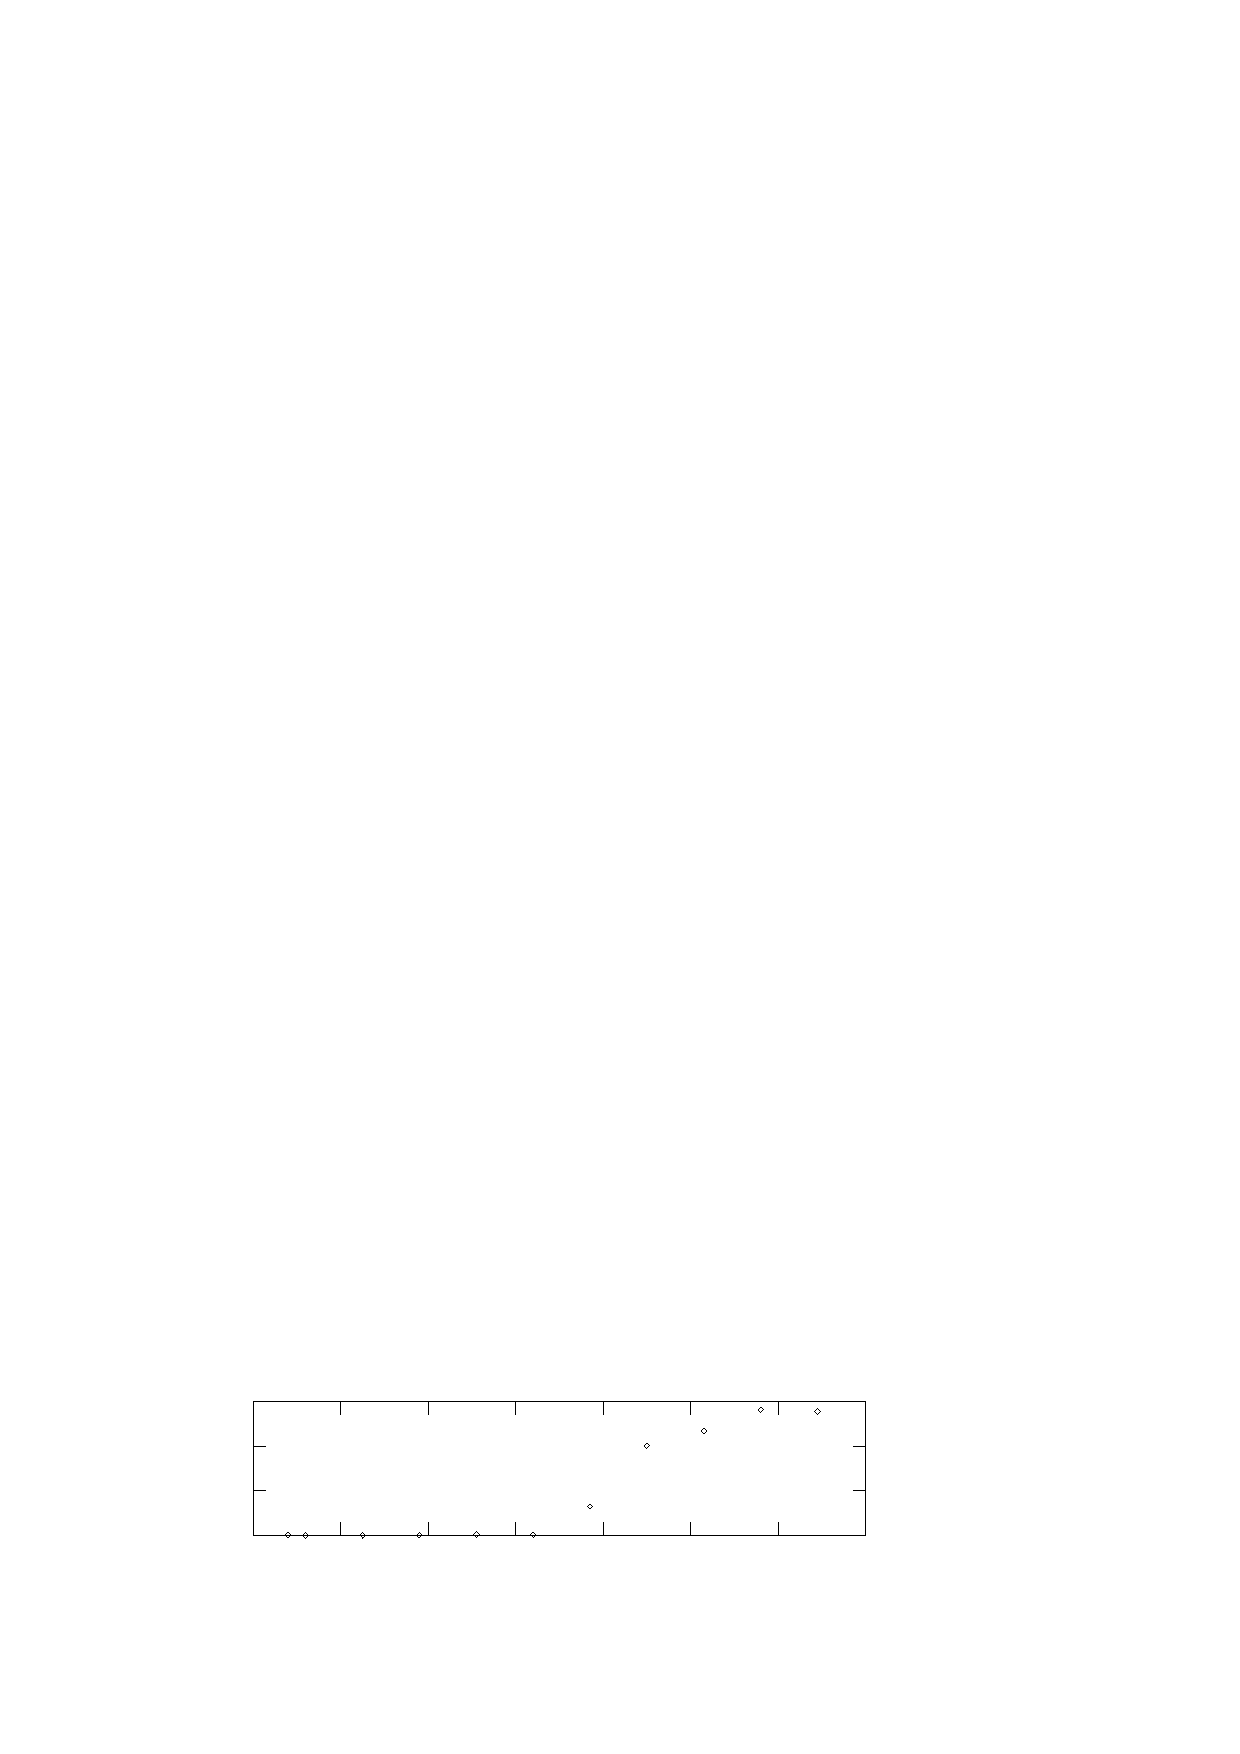
\includegraphics{Fo-equilibrium-amplitud-rounded-x}%
%\end{picture}%
%\begingroup
%\setlength{\unitlength}{0.0200bp}%
%\begin{picture}(18000,5400)(0,0)%
%\put(2200,1650){\makebox(0,0)[r]{\strut{}0.00}}%
%\put(2200,2717){\makebox(0,0)[r]{\strut{}0.50}}%
%\put(2200,3783){\makebox(0,0)[r]{\strut{}1.00}}%
%\put(2200,4850){\makebox(0,0)[r]{\strut{}1.50}}%
%\put(2475,1100){\makebox(0,0){\strut{}0.000}}%
%\put(4575,1100){\makebox(0,0){\strut{}0.001}}%
%\put(6675,1100){\makebox(0,0){\strut{}0.002}}%
%\put(8775,1100){\makebox(0,0){\strut{}0.003}}%
%\put(10875,1100){\makebox(0,0){\strut{}0.004}}%
%\put(12975,1100){\makebox(0,0){\strut{}0.005}}%
%\put(15075,1100){\makebox(0,0){\strut{}0.006}}%
%\put(17175,1100){\makebox(0,0){\strut{}0.007}}%
%\put(550,3250){\rotatebox{90}{\makebox(0,0){\strut{}$\sigma_x^\ast$}}}%
%\put(9825,275){\makebox(0,0){\strut{}$P_o^\ast$}}%
%\put(600,1000){\rotatebox{0}{\makebox(0,0){\strut{}(c)}}}%
%\end{picture}%
%\endgroup
%\endinput
